Now that we have a model that has trained for some length of time, we can try getting it to generate something new of its own. To do this, we need to feed it a section of seed audio to act as the first input. After generating on the seed, it will look back at its previous generated material and keep constructing recursively. To accomplish this, we will create a generator class similar to our trainer class that loads a trained model, the path to a seed, the path to the output file and some other attributes.

\begin{minted}{python}
import torch
import numpy as np
import os
from soundfile import write as write_wav

from WaveNet.Wavenet import *
import WaveNet.data as data

class Generator:
    def __init__(self, model, model_dir, step, sample_rate, seed_path, out_path, sample_size):
        """
        Args:
            model      (WaveNet) : Trained WaveNet model 
            model_dir     (path) : Path to the model's saved parameters
            step           (int) : The number of the model to load
            sample_rate    (int) : Sample rate at which to generate 
            seed_path     (path) : Path to the seed file 
            out_path      (path) : File path of output file 
            sample_size    (int) : Number of samples to generate
        """
        self.sample_rate = sample_rate
        self.sample_size = sample_size
        self.seed = seed_path
        self.out_path = out_path

        self.wavenet = model
        self.wavenet.load(model_dir, step)
\end{minted}

\newpage
Our generate method starts by companding and encoding the seed\footnote{The methods that do this in the \code{Generator} class are available in Appendix A} and then feeding it through the generate method. After the first one, it reassigns the input to whatever it just generated and repeats until the output is the requested length or, if none is given, two receptive fields.

\begin{minted}{python}
class Generator:
    ...
    def generate(self):
        """
        Generate from the given seed
        """
        outputs = []
        inputs, audio_length = self._get_seed_from_audio(self.seed)

        while True:
            new = self.wavenet.generate(inputs)
            
            # Not relevant but I love this syntax
            outputs = torch.cat((outputs, new), dim=1) if len(outputs) else new

            if len(outputs[0] >= audio_length):
                break
                
            # If not long enough, reassign input to whatever we just generated
            inputs = torch.cat((inputs[:, :-len(new[0]), :], new), dim=1)
        
        # Clip output to the desired length and save
        outputs = outputs[:, :audio_length, :]
        self._save_to_audio_file(outputs)
        
\end{minted}

With our \code{Generator} class, we just need a quick script to actually run.

\begin{minted}{python}
from WaveNet.Wavenet import WaveNet
from WaveNet.generator import Generator


if __name__ == '__main__':
        model = WaveNet(5, 10, 256, 512)

        for save_step in [2, 50, 100, 150, 200, 250, 300, 317]:
            outpath = './generator_output/gen_{}.wav'.format(save_step)
            generator = Generator(model, './model_saves',
                save_step, 16000, './data/helloworld.wav', outpath, 100000)
            generator.generate()

>>> python gen.py
Loading model from ./model_saves
94885/1668550 samples are generated.
Saved wav file at ./generator_output/gen_2.wav
Loading model from ./model_saves
94885/1668550 samples are generated.
...
\end{minted}

Listening to the samples, we get what sounds like rhythmic static. A keen ear will notice that that \code{gen\_2.wav} has more high end\footnote{I'd like to take this opportunity to thank Dr. Doug Bielmeier for forcing me to do ear training in Recording 1.}, and looking at the spectrograms in Figure \ref{fig:specgram}, we see \code{gen\_317.wav} is slightly darker in the areas between the breaks, indicated a lesser presence of frequency content there relative to the darker portions. The rhythmic nature of these examples is the most interesting feature, likely having been picked up by the model from the rhythmic nature of the seed file. This would mean that at this level of complexity and this amount of training, the model can at least pick up on broad structural features of the seed. For comparison when seeded with \code{arctic\_a0001.wav}, we do not see this rhythm, shown in \code{gen\_counter.wav}.

\begin{figure}[htbp]
    \centering
    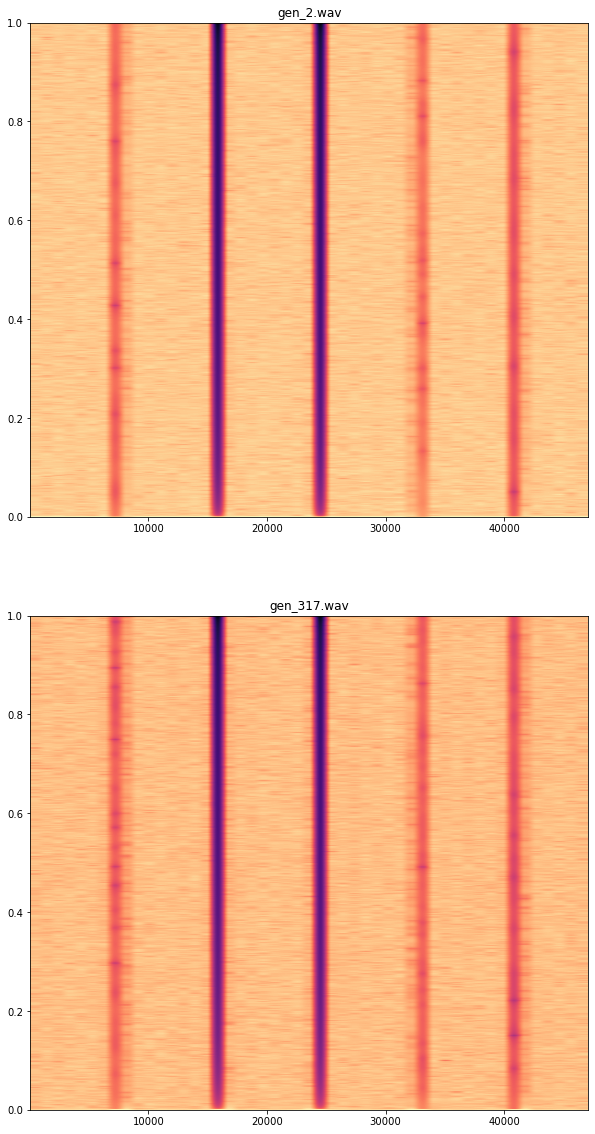
\includegraphics[width=3.5in]{images/spectrogram.png}
    \caption{Mel Spectrograms for \code{gen\_2.wav} and \code{gen\_317.wav}}
    \label{fig:specgram}
\end{figure}
